\documentclass[12pt,a4paper]{article}
\usepackage[utf8]{inputenc}
\usepackage[OT1]{fontenc}
\usepackage{amsmath}
\usepackage{amsfonts}
\usepackage{amssymb}
\usepackage{graphicx}
\usepackage{tikz}
\usepackage{pgfplotstable}
\usepackage{mathtext}

\usepackage[T1]{fontenc}
\usepackage[utf8]{inputenc}
\usepackage[english, bulgarian, russian]{babel}

\usepackage{tikz}
\usepackage{pgfplots}
\usepackage{indentfirst}
\usepackage[export]{adjustbox}
\usepackage{multirow}
\usepackage{geometry} \geometry{verbose,a4paper,tmargin=2cm,bmargin=2cm,lmargin=1.5cm,rmargin=1.5cm}

\graphicspath{{Images/}}
\usepackage[left=2cm,right=2cm,top=2cm,bottom=2cm]{geometry}
\usepackage{wrapfig}
\usepackage{setspace}
\usepackage{indentfirst}
\usepackage{subfigure}


\begin{document}

\begin{titlepage}
  \begin{center}
    \huge
    Московский Физико-технический Институт
    
    (Национальный исследовательский университет)
    \vspace{0.5cm}

   
    \vspace{0.25cm}
 
    \vfill
 
    \vfill

    \textsc{\bf{Отчет о выполнении работы 2.5.1}}\\[3mm]
    
    {\LARGE  Измерение коэффициента поверхностного натяжения жидкости}
  \bigskip
    \vfill
    
\end{center}
\vfill
\begin{flushright}

    Выполнили студентки 1 курса
    
    ФБМФ, группа Б06-103

    Попеску Полина
    
    
    Фитэль Алёна

\end{flushright}
\bigskip


\vfill

\begin{center}
  Долгопрудный, 2022 г.
\end{center}
\end{titlepage}

\section{Введение}

\textbf{Цель работы:} 1) измерение температурной зависимости  коэффициента поверхностного натяжения дистиллированной воды с использованием известного коэффициента поверхностного натяжения спирта;  2) определение полной поверхностной энергии  и теплоты, необходимой для изотермического образования единицы  поверхности жидкости  при различной температуре. 


\textbf{В работе используются:} прибор  Ребиндера  с термостатом и микроманометром; исследуемые жидкости; стаканы.


\section{Теоретический материал}

Наличие поверхностного слоя приводит к различию давлений по разные стороны от искривленной границы раздела двух сред.  Для сферического пузырька с воздухом  внутри жидкости избыточное давление даётся формулой Лапласа:

\begin{equation}
    \Delta P = P_{внутри} - P_{снаружи} = \frac{2\sigma}{r}
\end{equation}
где $\sigma$ – коэффициент поверхностного натяжения, $P_{внутри}$ и $P_{снаружи}$ – давление внутри пузырька и снаружи, $r$ – радиус кривизны поверхности раздела двух фаз. Эта формула лежит в основе предлагаемого метода определения коэффициента поверхностного натяжения жидкости. Измеряется давление $\DeltaP$, необходимое для выталкивания в жидкость пузырька воздуха.


\section{Экспериментальная установка}

Исследуемая жидкость (дистиллированная вода) наливается в сосуд (колбу) В (рис.1). Тестовая жидкость  (этиловый спирт) наливается  в сосуд Е.  При измерениях  колбы герметично закрываются  пробками.   Через одну из двух пробок  проходит полая металлическая игла С. Этой пробкой закрывается сосуд, в котором  проводятся измерения. Верхний конец иглы открыт в атмосферу, а нижний погружен в жидкость. Другой сосуд герметично закрывается второй пробкой. При создании достаточного  разряжения воздуха в колбе с иглой пузырьки воздуха начинают пробулькивать через жидкость. Поверхностное натяжение можно определить по величине разряжения $∆P$ (1), необходимого для прохождения пузырьков (при известном радиусе иглы).
Разряжение в системе создается с помощью аспиратора А. Кран К2 разделяет две полости аспиратора. Верхняя полость при закрытом кране К2  заполняется водой. Затем кран К2 открывают и заполняют водой  нижнюю полость  аспиратора.  Разряжение воздуха создается в нижней полости  при открывании крана К1, когда  вода вытекает из неё по каплям. В колбах В и С, соединённых трубками с нижней полостью аспиратора,  создается такое же пониженное давление. Разность давлений в полостях с разряженным воздухом и атмосферой измеряется спиртовым микроманометром (устройство микроманометра описано в Приложении). 
Для стабилизации температуры исследуемой жидкости через рубашку D колбы В непрерывно прогоняется вода из термостата.

\begin{figure}[h!]
    \centering
    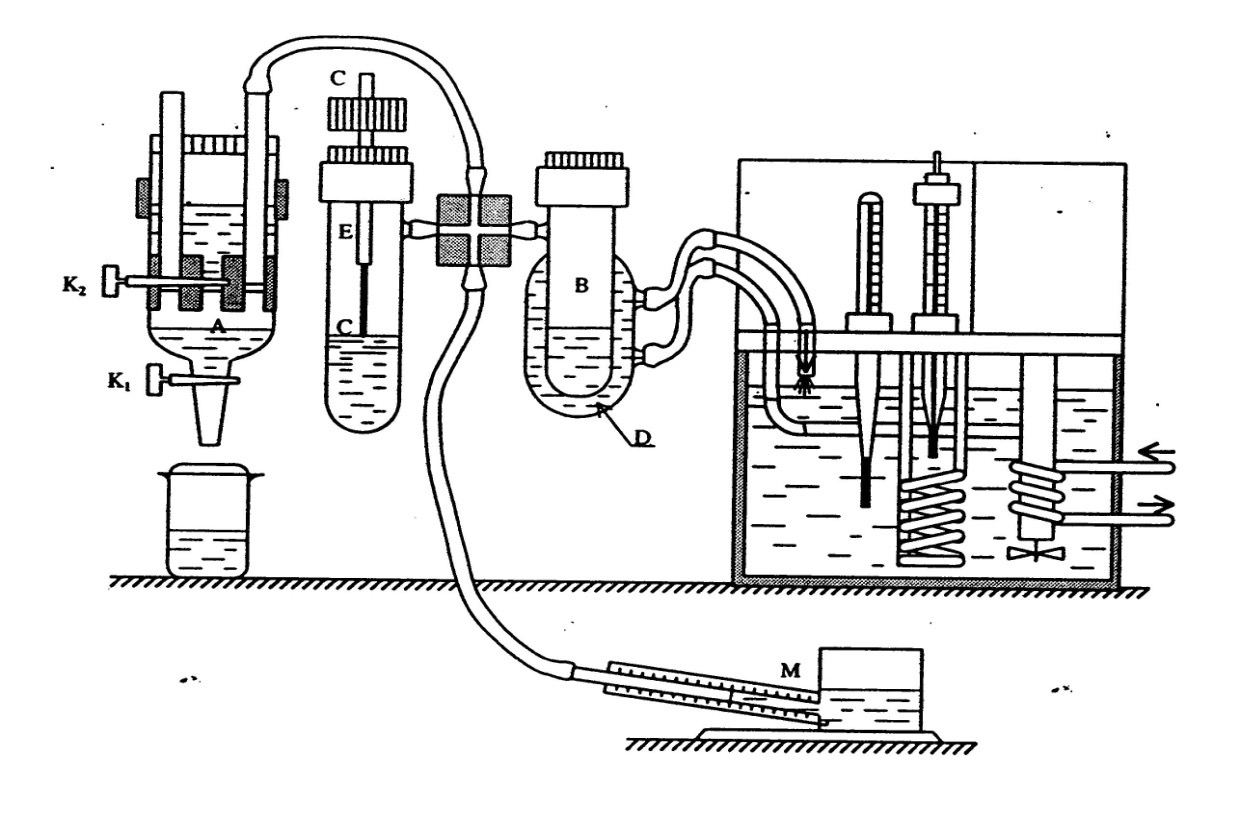
\includegraphics[scale=0.3]{ust.jpeg}
    \caption{Схема установки для измерения температурной зависимости коэффициента поверхностного натяжения}
\end{figure}

Обычно кончик иглы лишь касается поверхности жидкости, чтобы исключить влияние гидростатического давления столба жидкости. Однако при измерении температурной зависимости коэффициента поверхностного натяжения возникает ряд сложностей. Во-первых, большая теплопроводность металлической трубки приводит к тому, что температура на конце трубки заметно ниже, чем в глубине жидкости. Во-вторых, тепловое расширение поднимает уровень жидкости при увеличении температуры. 
Обе погрешности можно устранить, погрузив кончик трубки до самого дна. Полное давление, измеренное при этом микроманометром, $P = ∆P + \rho gh$.

\newpage

Заметим, что $\rho gh$ от температуры практически не зависит, так как подъём уровня жидкости компенсируется уменьшением её плотности (произведение $\rho gh$ определяется массой всей жидкости и поэтому постоянно). Величину  $\rho gh$ следует измерить двумя способами. Во-первых, замерить величину $P1= ∆P'$, когда кончик трубки только касается поверхности жидкости. Затем при этой же температуре опустить иглу до дна и замерить $P2= \rho gh + ∆P"$ ($∆P', ∆P"$ – давление Лапласа). Из-за  несжимаемости  жидкости можно положить $∆P'= ∆P "$ и тогда $\rho gh = P2-P1$. Во-вторых, при измерениях $P1$ и $P2$ замерить линейкой  глубину погружения иглы $h$. Это можно сделать, замеряя расстояние между верхним концом иглы и любой неподвижной частью прибора при положении иглы на поверхности и в глубине колбы.

В частности подобную же операцию необходимо сделать и при заполнении водой аспиратора А. В противном случае при заполнении аспиратора водой давление воздуха в системе повышается, спирт из трубки микроманометра выдавливается, в узлах соединений микроманометра образуются воздушные пузыри. Наличие этих пузырей приводит к полному нарушению калибровки манометра и невоспроизводимости измерений.


\section{Обработка результатов измерений}
\begin{enumerate}
    \item Проверим герметичность установки. Для этого заполним аспиратор водой. Чистую сухую иглу установим в сосуд со спиртом так, чтобы кончик иглы лишь касался поверхности спирта. Плотно закроем обе колбы В и Е пробками. Откроем кран $К_1$ аспиратора и добьемся пробулькивания пузырьков воздуха в колбе. Замерим показания микроманометра. Закроем кран $К_1$. Наблюдаем за показаниями манометра: при отсутствии течи в установке столбик спирта в манометре неподвижен. 
    
    \item Убедившись в герметичности системы, начнем измерения. Откроем кран $К_1$. Подберем частоту падения капель из аспиратора так, чтобы максимальное давление манометра не зависело от этой частоты (не чаще, чем 1 капля в 5 секунд).
    \newpage

    \item Измерим максимальное давление $\Delta P_{спирт}$ при  пробулькивании пузырьков воздуха через спирт. По разбросу результатов оценим случайную погрешность измерения. Пользуясь табличным значением коэффициента поверхностного натяжения спирта, определим по формуле (1) диаметр иглы, приняв значение $\sigma_{спирт} $ при $T=20^oC$ равным $22,8 \cdot 10^{-3}\ Н/м$. Сравним полученный результат с диаметром иглы, измеренным по микроскопу.
    
    \begin{table}[ht]
        \centering
        \begin{tabular}{|c|c|c|c|}
            \hline
            $\Delta P$, Па & $\sigma_P$, Па & $d$, мм & $\sigma_d$, мм \\
            \hline
             92,2 & 2,0 & 0,99& 0,03\\
             \hline
        \end{tabular}
        \caption{Диаметр иглы при измерении $\Delta P$}
        \label{tab:my_label}
    \end{table}

    Значение диаметра иглы, полученное через микроскоп, в пределах погрешности совпадает с расчитанным: $d = (1,00 \pm 0,05)\ мм$.
    
    \item Перенесем предварительно промытую и просушенную от спирта иглу в колбу с дистиллированной водой. Измерим максимальное давление $Р_1$ при пробулькивании пузырьков, когда игла лишь касается поверхности воды. Аспиратор должен быть предварительно  заполнен водой почти доверху. Отрегулируем скорость поднятия уровня спирта в манометре и сохраним её в течение всех экспериментов. Измерим расстояние между верхним концом иглы и любой неподвижной частью прибора $h_1$.
    
    \item Утопим иглу до предела (между концом иглы и дном необходимо оставить небольшой зазор, чтобы образующийся пузырёк не касался дна). Измерим $h_2$ (как в пункте 4) и максимальное давление в пузырьках $Р_2$.
    По разности давлений $\Delta Р = Р_2 - Р_1$ определим глубину погружения $\Delta h$ иглы и сравним с $\Delta h =  h_1- h_2$.
    
    \begin{table}[ht]
        \centering
        \begin{tabular}{|c|c|c|c|c|c|c|}
            \hline
             $P_1$, Па & $P_2$, Па & $\sigma_P$, Па & $\Delta P$, Па & $\sigma_{\Delta P}$, Па & $\Delta h$, см & $\sigma_{\Delta h}$,  см \\
             \hline
             262,4& 366,0& 2,0 & 104&3 & 1,06& 0,03\\
             \hline 
        \end{tabular}
        \caption{Глубина погружения через разницу давлений}
    \end{table}
    
    \begin{table}[ht]
        \centering
        \begin{tabular}{|c|c|c|c|c|}
        \hline
            $h_1$, см & $h_2$, см & $\sigma_h$, см & $\Delta h$, см & $\sigma_{\Delta h}$, см  \\
            \hline
             6,1& 5,0 & 0,1&1,10 & 0,14\\
            \hline
        \end{tabular}
        \caption{Измерение глубины погружения}
    \end{table}

    Полученные разными методами данные о глубине погружения иглы отличаются друг от друга в пределах погрешности. При дальнейших измерениях, будем использовать значение, полученное экспериментально, так как его относительная погрешность ($\epsilon=2,8
    \%$) меньше, чем погрешность измерения глубины погружения, измереннная с помощью линейки ($\epsilon=13\%$).
    
    \item Снимем температурную зависимость $\sigma (Т)$ дистиллированной воды. 
    Для этого включим термостат и подождем, пока нужная вам температура не стабилизируется. 
    После этого проведем измерение давления. 
    Для уменьшения погрешности опыта замер давления при фиксированной температуре проводим несколько раз. 
    Проводить измерение температурной зависимости  рекомендуется в диапазоне  $25^oС - 55^oС$ через $5^oC$. Оценим погрешность измерения давления и температуры. Рассчитаем величину коэффициента поверхностного натяжения воды $\sigma (T)$, используя значение диаметра иглы, полученное при измерениях на спирте (относительная погрешность при это способе измерения($\epsilon=3\%$) меньше, чем относительная погрешность измерения с помощью микроскопа($\epsilon=5\%$)). 
      \begin{table}[ht]
        \centering
        \begin{tabular}{|c|c|c|c|c|c|}
        \hline
            $T,\ ^oC$ & $\sigma_T,\ ^oC$ & $\Delta P$, Па & $\sigma_P$, Па & $\sigma(T),\ 10^{-3}$, Н/м & $\sigma_{\sigma},\ 10^{-3}$ Н/м\\
            \hline
            25,2 & 0,2& 262 & 4&90 & 5\\
            \hline
            30,4 & 0,2& 259 & 4&90& 5\\
            \hline
            35,2 & 0,2& 255 & 4& 90& 5\\
            \hline
            40,0 & 0,2& 251&4 & 88& 4\\
            \hline
            45,1 & 0,2& 248 &4 & 87& 4\\
            \hline
            50,0 & 0,2& 244 & 4& 86& 4\\
            \hline
            55,0 &0,2&243 & 4& 85& 4\\
            \hline
        \end{tabular}
        \caption{Измерение коэффициента поверхностного натяжения воды}
    \end{table}
    
    \item Построем график зависимости $\sigma (T)$ и определим по графику температурный коэффициент $d\sigma / d T$. 
    
    По МНК получаем, что коэффициент наклона $\frac {d\sigma}{dT} = (-0,238\pm 0,009)\ \frac {мН}{м\cdot К}$. Табличное значение $\frac {d\sigma}{dT} = -0,160 \frac {мН}{м\cdot К}$.
    
    
  \begin{figure}[h!]
    \centering
    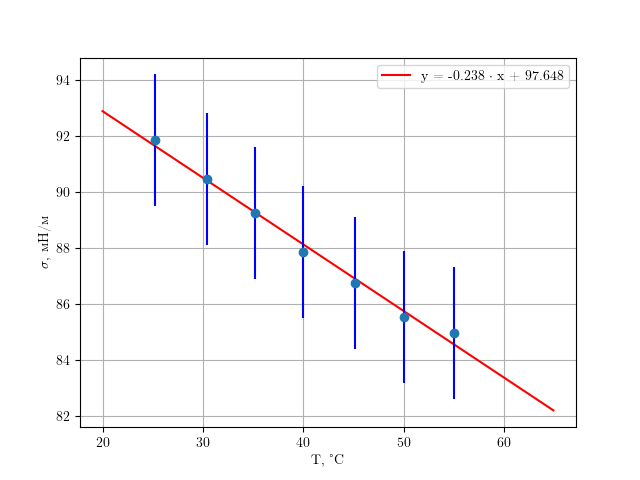
\includegraphics[scale=1]{sigma(T).png}
    \caption {График зависимости $\sigma(T)$}
\end{figure}
    
    \item Построим график зависимости от температуры теплоты образования единицы поверхности жидкости $q = -T\cdot d\sigma/dT$ и график зависимости от температуры поверхностной энергии $U$ единицы площади $F$:\ $U/F = (\sigma - T \cdot d \sigma/dT)$.  Значение $U/F$ постоянно и равно $(162,6 \pm 2,4)\ \frac {мН}{м\cdot К}$.
  
    
     \begin{figure}[h!]
    \centering
    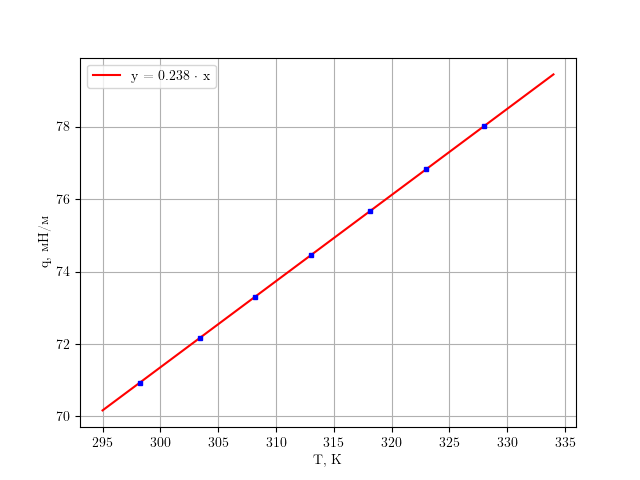
\includegraphics[scale=0.75]{q(T).png}
    \caption {График зависимости $q(T)$}
\end{figure}
    
     
        \begin{figure}[h!]
    \centering
    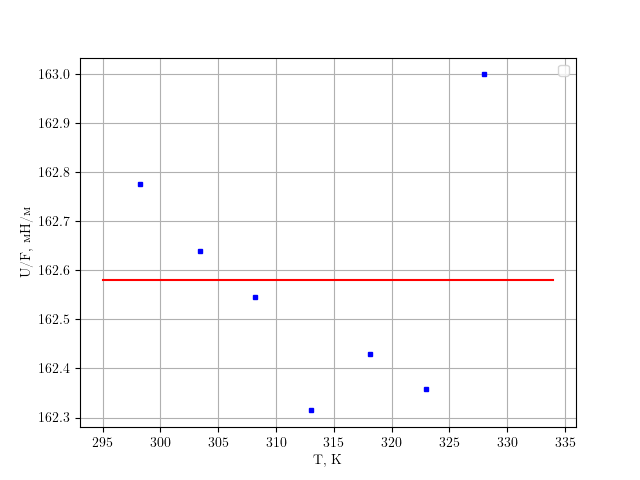
\includegraphics[scale=0.75]{UF(T).png}
    \caption {График зависимости $U/F (T)$}
\end{figure}
\end{enumerate}



\section{Обсуждение результатов и выводы}


\item В ходе данной лабораторной работы мы исследовали температурную зависимость коэффициента поверхностного натяжения дистиллированной воды от температуры. Полученная зависимость оказалась линейной в интервале рабочих температур от 25$^\circ$C до 55$^\circ$C.Полученный результат вполне естественен, потому что с увеличением температуры интенсивность межмолекулярного взаимодействия уменьшается, вследствие чего снижается и поверхностное натяжение жидкостей на границе с воздухом или с собственным паром. Вдали от критической температуры поверхностное натяжение уменьшается прямо пропорционально росту температуры. Стоит отметить, что наш результат в пределах погрешности не  совпадает с табличным значением. Это обуславливается несколькими факторами. Во-первых, диаметр образующихся пузырей не обязан совпадать с диаметром иглы. Во-вторых, температура термостата не совпадает в реальности с температурой воды вследствие теплового взаимодействия колбы с окружающей средой. В-третьих, тепловое расширение поднимает уровень жидкости, вследствие чего увеличивается добавочное давление $\rho gh$, и тогда $\Delta P$ уменьшается. Из этого следует, что расчитываемое нами по формуле Лапласа (1) поверхностное натяжение должно уменьшится. В-четвертых, большую погрешность мог внести тот факт, что исследуемая в ходе эксперимента <<дистиллированная>> вода, имела примеси спирта, которые попали туда в результате некачественной очистки иглы от остатков этанола после первой части работы. Поэтому полученные значения  для поверхностного натяжения  разумно интерпретировать как значения поверхностного натяжения раствора, а не чистого вещества.
\item Зная температурный коэффициент поверхностного натяжения, можно исследовать зависимость теплоты образования единицы поверхности жидкости $q = q(T)$ и поверхностной энергии единицы площади $U/\Pi$ от температуры. Если коэффициент поверхностного натяжения линейно зависит от температуры, то функция $q =-T\frac{d\sigma}{dT}$ является линейной, что отражено на графике зависимости $q(T)$.
\item Для теоретического подтверждения экспериментального результата, показывающего независимость внутренней энергии поверхности $U/\Pi$ от температуры, запишем уравнение Гиббса-Гельмгольца для поверхностного слоя: $U/\Pi = \sigma - T\frac{d\sigma}{dT}$. Продифференцируем его по температуре: $\frac{\partial U/\Pi}{\partial T} = -T \frac{\partial^2 \sigma}{\partial T^2}$. Так как первая производная $\sigma$ по $T$ есть величина постоянная, то вторая производная равна нулю, следовательно, внутренняя энергия поверхностного слоя не зависит от температуры, что хорошо отражает график $U/F (T)$.




\end{document}





















  begin{figure}[h]
\begin{minipage}[h]{0.52\linewidth}
\center{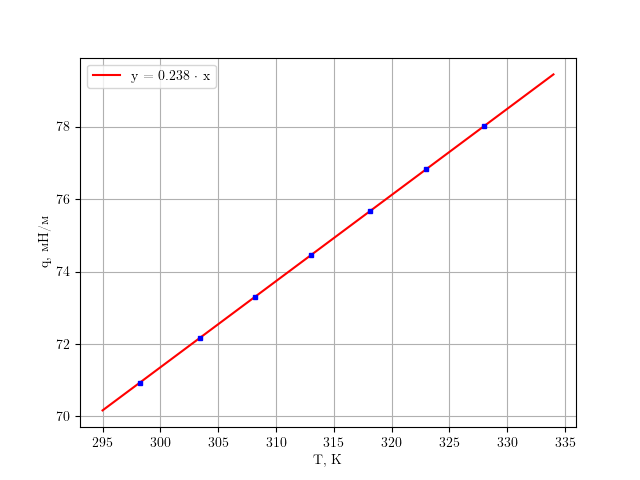
\includegraphics[width=1\linewidth]{q(T).png} \\ График зависимости $q(T)$}
\end{minipage}
\hfill
\begin{minipage}[h]{0.52\linewidth}
\center{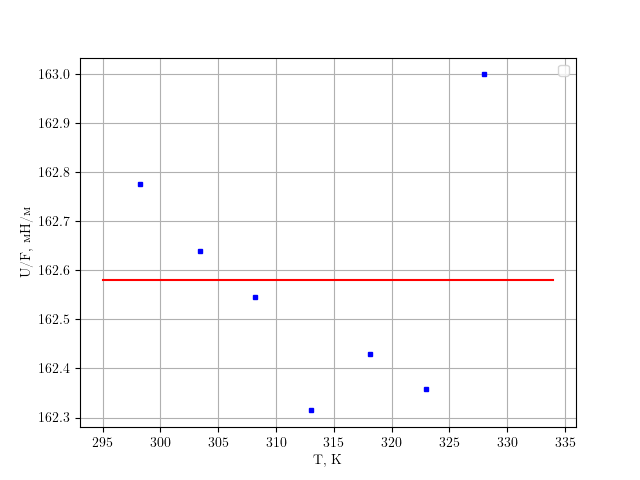
\includegraphics[width=1\linewidth]{UF(T).png} \\ График зависимости $U/F (T)$}
\end{minipage}
\label{ris:image1}
\end{figure}